
% Default to the notebook output style

    


% Inherit from the specified cell style.




    
\documentclass[11pt]{article}

    
    
    \usepackage[T1]{fontenc}
    % Nicer default font (+ math font) than Computer Modern for most use cases
    \usepackage{mathpazo}

    % Basic figure setup, for now with no caption control since it's done
    % automatically by Pandoc (which extracts ![](path) syntax from Markdown).
    \usepackage{graphicx}
    % We will generate all images so they have a width \maxwidth. This means
    % that they will get their normal width if they fit onto the page, but
    % are scaled down if they would overflow the margins.
    \makeatletter
    \def\maxwidth{\ifdim\Gin@nat@width>\linewidth\linewidth
    \else\Gin@nat@width\fi}
    \makeatother
    \let\Oldincludegraphics\includegraphics
    % Set max figure width to be 80% of text width, for now hardcoded.
    \renewcommand{\includegraphics}[1]{\Oldincludegraphics[width=.8\maxwidth]{#1}}
    % Ensure that by default, figures have no caption (until we provide a
    % proper Figure object with a Caption API and a way to capture that
    % in the conversion process - todo).
    \usepackage{caption}
    \DeclareCaptionLabelFormat{nolabel}{}
    \captionsetup{labelformat=nolabel}

    \usepackage{adjustbox} % Used to constrain images to a maximum size 
    \usepackage{xcolor} % Allow colors to be defined
    \usepackage{enumerate} % Needed for markdown enumerations to work
    \usepackage{geometry} % Used to adjust the document margins
    \usepackage{amsmath} % Equations
    \usepackage{amssymb} % Equations
    \usepackage{textcomp} % defines textquotesingle
    % Hack from http://tex.stackexchange.com/a/47451/13684:
    \AtBeginDocument{%
        \def\PYZsq{\textquotesingle}% Upright quotes in Pygmentized code
    }
    \usepackage{upquote} % Upright quotes for verbatim code
    \usepackage{eurosym} % defines \euro
    \usepackage[mathletters]{ucs} % Extended unicode (utf-8) support
    \usepackage[utf8x]{inputenc} % Allow utf-8 characters in the tex document
    \usepackage{fancyvrb} % verbatim replacement that allows latex
    \usepackage{grffile} % extends the file name processing of package graphics 
                         % to support a larger range 
    % The hyperref package gives us a pdf with properly built
    % internal navigation ('pdf bookmarks' for the table of contents,
    % internal cross-reference links, web links for URLs, etc.)
    \usepackage{hyperref}
    \usepackage{longtable} % longtable support required by pandoc >1.10
    \usepackage{booktabs}  % table support for pandoc > 1.12.2
    \usepackage[inline]{enumitem} % IRkernel/repr support (it uses the enumerate* environment)
    \usepackage[normalem]{ulem} % ulem is needed to support strikethroughs (\sout)
                                % normalem makes italics be italics, not underlines
    

    
    
    % Colors for the hyperref package
    \definecolor{urlcolor}{rgb}{0,.145,.698}
    \definecolor{linkcolor}{rgb}{.71,0.21,0.01}
    \definecolor{citecolor}{rgb}{.12,.54,.11}

    % ANSI colors
    \definecolor{ansi-black}{HTML}{3E424D}
    \definecolor{ansi-black-intense}{HTML}{282C36}
    \definecolor{ansi-red}{HTML}{E75C58}
    \definecolor{ansi-red-intense}{HTML}{B22B31}
    \definecolor{ansi-green}{HTML}{00A250}
    \definecolor{ansi-green-intense}{HTML}{007427}
    \definecolor{ansi-yellow}{HTML}{DDB62B}
    \definecolor{ansi-yellow-intense}{HTML}{B27D12}
    \definecolor{ansi-blue}{HTML}{208FFB}
    \definecolor{ansi-blue-intense}{HTML}{0065CA}
    \definecolor{ansi-magenta}{HTML}{D160C4}
    \definecolor{ansi-magenta-intense}{HTML}{A03196}
    \definecolor{ansi-cyan}{HTML}{60C6C8}
    \definecolor{ansi-cyan-intense}{HTML}{258F8F}
    \definecolor{ansi-white}{HTML}{C5C1B4}
    \definecolor{ansi-white-intense}{HTML}{A1A6B2}

    % commands and environments needed by pandoc snippets
    % extracted from the output of `pandoc -s`
    \providecommand{\tightlist}{%
      \setlength{\itemsep}{0pt}\setlength{\parskip}{0pt}}
    \DefineVerbatimEnvironment{Highlighting}{Verbatim}{commandchars=\\\{\}}
    % Add ',fontsize=\small' for more characters per line
    \newenvironment{Shaded}{}{}
    \newcommand{\KeywordTok}[1]{\textcolor[rgb]{0.00,0.44,0.13}{\textbf{{#1}}}}
    \newcommand{\DataTypeTok}[1]{\textcolor[rgb]{0.56,0.13,0.00}{{#1}}}
    \newcommand{\DecValTok}[1]{\textcolor[rgb]{0.25,0.63,0.44}{{#1}}}
    \newcommand{\BaseNTok}[1]{\textcolor[rgb]{0.25,0.63,0.44}{{#1}}}
    \newcommand{\FloatTok}[1]{\textcolor[rgb]{0.25,0.63,0.44}{{#1}}}
    \newcommand{\CharTok}[1]{\textcolor[rgb]{0.25,0.44,0.63}{{#1}}}
    \newcommand{\StringTok}[1]{\textcolor[rgb]{0.25,0.44,0.63}{{#1}}}
    \newcommand{\CommentTok}[1]{\textcolor[rgb]{0.38,0.63,0.69}{\textit{{#1}}}}
    \newcommand{\OtherTok}[1]{\textcolor[rgb]{0.00,0.44,0.13}{{#1}}}
    \newcommand{\AlertTok}[1]{\textcolor[rgb]{1.00,0.00,0.00}{\textbf{{#1}}}}
    \newcommand{\FunctionTok}[1]{\textcolor[rgb]{0.02,0.16,0.49}{{#1}}}
    \newcommand{\RegionMarkerTok}[1]{{#1}}
    \newcommand{\ErrorTok}[1]{\textcolor[rgb]{1.00,0.00,0.00}{\textbf{{#1}}}}
    \newcommand{\NormalTok}[1]{{#1}}
    
    % Additional commands for more recent versions of Pandoc
    \newcommand{\ConstantTok}[1]{\textcolor[rgb]{0.53,0.00,0.00}{{#1}}}
    \newcommand{\SpecialCharTok}[1]{\textcolor[rgb]{0.25,0.44,0.63}{{#1}}}
    \newcommand{\VerbatimStringTok}[1]{\textcolor[rgb]{0.25,0.44,0.63}{{#1}}}
    \newcommand{\SpecialStringTok}[1]{\textcolor[rgb]{0.73,0.40,0.53}{{#1}}}
    \newcommand{\ImportTok}[1]{{#1}}
    \newcommand{\DocumentationTok}[1]{\textcolor[rgb]{0.73,0.13,0.13}{\textit{{#1}}}}
    \newcommand{\AnnotationTok}[1]{\textcolor[rgb]{0.38,0.63,0.69}{\textbf{\textit{{#1}}}}}
    \newcommand{\CommentVarTok}[1]{\textcolor[rgb]{0.38,0.63,0.69}{\textbf{\textit{{#1}}}}}
    \newcommand{\VariableTok}[1]{\textcolor[rgb]{0.10,0.09,0.49}{{#1}}}
    \newcommand{\ControlFlowTok}[1]{\textcolor[rgb]{0.00,0.44,0.13}{\textbf{{#1}}}}
    \newcommand{\OperatorTok}[1]{\textcolor[rgb]{0.40,0.40,0.40}{{#1}}}
    \newcommand{\BuiltInTok}[1]{{#1}}
    \newcommand{\ExtensionTok}[1]{{#1}}
    \newcommand{\PreprocessorTok}[1]{\textcolor[rgb]{0.74,0.48,0.00}{{#1}}}
    \newcommand{\AttributeTok}[1]{\textcolor[rgb]{0.49,0.56,0.16}{{#1}}}
    \newcommand{\InformationTok}[1]{\textcolor[rgb]{0.38,0.63,0.69}{\textbf{\textit{{#1}}}}}
    \newcommand{\WarningTok}[1]{\textcolor[rgb]{0.38,0.63,0.69}{\textbf{\textit{{#1}}}}}
    
    
    % Define a nice break command that doesn't care if a line doesn't already
    % exist.
    \def\br{\hspace*{\fill} \\* }
    % Math Jax compatability definitions
    \def\gt{>}
    \def\lt{<}
    % Document parameters
    \title{Wholesale Customers Analysis}
    
    
    

    % Pygments definitions
    
\makeatletter
\def\PY@reset{\let\PY@it=\relax \let\PY@bf=\relax%
    \let\PY@ul=\relax \let\PY@tc=\relax%
    \let\PY@bc=\relax \let\PY@ff=\relax}
\def\PY@tok#1{\csname PY@tok@#1\endcsname}
\def\PY@toks#1+{\ifx\relax#1\empty\else%
    \PY@tok{#1}\expandafter\PY@toks\fi}
\def\PY@do#1{\PY@bc{\PY@tc{\PY@ul{%
    \PY@it{\PY@bf{\PY@ff{#1}}}}}}}
\def\PY#1#2{\PY@reset\PY@toks#1+\relax+\PY@do{#2}}

\expandafter\def\csname PY@tok@sh\endcsname{\def\PY@tc##1{\textcolor[rgb]{0.73,0.13,0.13}{##1}}}
\expandafter\def\csname PY@tok@s2\endcsname{\def\PY@tc##1{\textcolor[rgb]{0.73,0.13,0.13}{##1}}}
\expandafter\def\csname PY@tok@vm\endcsname{\def\PY@tc##1{\textcolor[rgb]{0.10,0.09,0.49}{##1}}}
\expandafter\def\csname PY@tok@s\endcsname{\def\PY@tc##1{\textcolor[rgb]{0.73,0.13,0.13}{##1}}}
\expandafter\def\csname PY@tok@se\endcsname{\let\PY@bf=\textbf\def\PY@tc##1{\textcolor[rgb]{0.73,0.40,0.13}{##1}}}
\expandafter\def\csname PY@tok@go\endcsname{\def\PY@tc##1{\textcolor[rgb]{0.53,0.53,0.53}{##1}}}
\expandafter\def\csname PY@tok@gr\endcsname{\def\PY@tc##1{\textcolor[rgb]{1.00,0.00,0.00}{##1}}}
\expandafter\def\csname PY@tok@cm\endcsname{\let\PY@it=\textit\def\PY@tc##1{\textcolor[rgb]{0.25,0.50,0.50}{##1}}}
\expandafter\def\csname PY@tok@mi\endcsname{\def\PY@tc##1{\textcolor[rgb]{0.40,0.40,0.40}{##1}}}
\expandafter\def\csname PY@tok@nb\endcsname{\def\PY@tc##1{\textcolor[rgb]{0.00,0.50,0.00}{##1}}}
\expandafter\def\csname PY@tok@c\endcsname{\let\PY@it=\textit\def\PY@tc##1{\textcolor[rgb]{0.25,0.50,0.50}{##1}}}
\expandafter\def\csname PY@tok@dl\endcsname{\def\PY@tc##1{\textcolor[rgb]{0.73,0.13,0.13}{##1}}}
\expandafter\def\csname PY@tok@m\endcsname{\def\PY@tc##1{\textcolor[rgb]{0.40,0.40,0.40}{##1}}}
\expandafter\def\csname PY@tok@ss\endcsname{\def\PY@tc##1{\textcolor[rgb]{0.10,0.09,0.49}{##1}}}
\expandafter\def\csname PY@tok@mb\endcsname{\def\PY@tc##1{\textcolor[rgb]{0.40,0.40,0.40}{##1}}}
\expandafter\def\csname PY@tok@kr\endcsname{\let\PY@bf=\textbf\def\PY@tc##1{\textcolor[rgb]{0.00,0.50,0.00}{##1}}}
\expandafter\def\csname PY@tok@kn\endcsname{\let\PY@bf=\textbf\def\PY@tc##1{\textcolor[rgb]{0.00,0.50,0.00}{##1}}}
\expandafter\def\csname PY@tok@gt\endcsname{\def\PY@tc##1{\textcolor[rgb]{0.00,0.27,0.87}{##1}}}
\expandafter\def\csname PY@tok@nl\endcsname{\def\PY@tc##1{\textcolor[rgb]{0.63,0.63,0.00}{##1}}}
\expandafter\def\csname PY@tok@s1\endcsname{\def\PY@tc##1{\textcolor[rgb]{0.73,0.13,0.13}{##1}}}
\expandafter\def\csname PY@tok@fm\endcsname{\def\PY@tc##1{\textcolor[rgb]{0.00,0.00,1.00}{##1}}}
\expandafter\def\csname PY@tok@bp\endcsname{\def\PY@tc##1{\textcolor[rgb]{0.00,0.50,0.00}{##1}}}
\expandafter\def\csname PY@tok@sc\endcsname{\def\PY@tc##1{\textcolor[rgb]{0.73,0.13,0.13}{##1}}}
\expandafter\def\csname PY@tok@mo\endcsname{\def\PY@tc##1{\textcolor[rgb]{0.40,0.40,0.40}{##1}}}
\expandafter\def\csname PY@tok@ne\endcsname{\let\PY@bf=\textbf\def\PY@tc##1{\textcolor[rgb]{0.82,0.25,0.23}{##1}}}
\expandafter\def\csname PY@tok@mh\endcsname{\def\PY@tc##1{\textcolor[rgb]{0.40,0.40,0.40}{##1}}}
\expandafter\def\csname PY@tok@nv\endcsname{\def\PY@tc##1{\textcolor[rgb]{0.10,0.09,0.49}{##1}}}
\expandafter\def\csname PY@tok@il\endcsname{\def\PY@tc##1{\textcolor[rgb]{0.40,0.40,0.40}{##1}}}
\expandafter\def\csname PY@tok@na\endcsname{\def\PY@tc##1{\textcolor[rgb]{0.49,0.56,0.16}{##1}}}
\expandafter\def\csname PY@tok@gs\endcsname{\let\PY@bf=\textbf}
\expandafter\def\csname PY@tok@gd\endcsname{\def\PY@tc##1{\textcolor[rgb]{0.63,0.00,0.00}{##1}}}
\expandafter\def\csname PY@tok@kd\endcsname{\let\PY@bf=\textbf\def\PY@tc##1{\textcolor[rgb]{0.00,0.50,0.00}{##1}}}
\expandafter\def\csname PY@tok@ch\endcsname{\let\PY@it=\textit\def\PY@tc##1{\textcolor[rgb]{0.25,0.50,0.50}{##1}}}
\expandafter\def\csname PY@tok@nd\endcsname{\def\PY@tc##1{\textcolor[rgb]{0.67,0.13,1.00}{##1}}}
\expandafter\def\csname PY@tok@nc\endcsname{\let\PY@bf=\textbf\def\PY@tc##1{\textcolor[rgb]{0.00,0.00,1.00}{##1}}}
\expandafter\def\csname PY@tok@gu\endcsname{\let\PY@bf=\textbf\def\PY@tc##1{\textcolor[rgb]{0.50,0.00,0.50}{##1}}}
\expandafter\def\csname PY@tok@sb\endcsname{\def\PY@tc##1{\textcolor[rgb]{0.73,0.13,0.13}{##1}}}
\expandafter\def\csname PY@tok@si\endcsname{\let\PY@bf=\textbf\def\PY@tc##1{\textcolor[rgb]{0.73,0.40,0.53}{##1}}}
\expandafter\def\csname PY@tok@cp\endcsname{\def\PY@tc##1{\textcolor[rgb]{0.74,0.48,0.00}{##1}}}
\expandafter\def\csname PY@tok@kp\endcsname{\def\PY@tc##1{\textcolor[rgb]{0.00,0.50,0.00}{##1}}}
\expandafter\def\csname PY@tok@nt\endcsname{\let\PY@bf=\textbf\def\PY@tc##1{\textcolor[rgb]{0.00,0.50,0.00}{##1}}}
\expandafter\def\csname PY@tok@sx\endcsname{\def\PY@tc##1{\textcolor[rgb]{0.00,0.50,0.00}{##1}}}
\expandafter\def\csname PY@tok@gh\endcsname{\let\PY@bf=\textbf\def\PY@tc##1{\textcolor[rgb]{0.00,0.00,0.50}{##1}}}
\expandafter\def\csname PY@tok@vi\endcsname{\def\PY@tc##1{\textcolor[rgb]{0.10,0.09,0.49}{##1}}}
\expandafter\def\csname PY@tok@kt\endcsname{\def\PY@tc##1{\textcolor[rgb]{0.69,0.00,0.25}{##1}}}
\expandafter\def\csname PY@tok@w\endcsname{\def\PY@tc##1{\textcolor[rgb]{0.73,0.73,0.73}{##1}}}
\expandafter\def\csname PY@tok@sr\endcsname{\def\PY@tc##1{\textcolor[rgb]{0.73,0.40,0.53}{##1}}}
\expandafter\def\csname PY@tok@mf\endcsname{\def\PY@tc##1{\textcolor[rgb]{0.40,0.40,0.40}{##1}}}
\expandafter\def\csname PY@tok@sa\endcsname{\def\PY@tc##1{\textcolor[rgb]{0.73,0.13,0.13}{##1}}}
\expandafter\def\csname PY@tok@ge\endcsname{\let\PY@it=\textit}
\expandafter\def\csname PY@tok@ow\endcsname{\let\PY@bf=\textbf\def\PY@tc##1{\textcolor[rgb]{0.67,0.13,1.00}{##1}}}
\expandafter\def\csname PY@tok@cpf\endcsname{\let\PY@it=\textit\def\PY@tc##1{\textcolor[rgb]{0.25,0.50,0.50}{##1}}}
\expandafter\def\csname PY@tok@vg\endcsname{\def\PY@tc##1{\textcolor[rgb]{0.10,0.09,0.49}{##1}}}
\expandafter\def\csname PY@tok@gp\endcsname{\let\PY@bf=\textbf\def\PY@tc##1{\textcolor[rgb]{0.00,0.00,0.50}{##1}}}
\expandafter\def\csname PY@tok@kc\endcsname{\let\PY@bf=\textbf\def\PY@tc##1{\textcolor[rgb]{0.00,0.50,0.00}{##1}}}
\expandafter\def\csname PY@tok@nn\endcsname{\let\PY@bf=\textbf\def\PY@tc##1{\textcolor[rgb]{0.00,0.00,1.00}{##1}}}
\expandafter\def\csname PY@tok@ni\endcsname{\let\PY@bf=\textbf\def\PY@tc##1{\textcolor[rgb]{0.60,0.60,0.60}{##1}}}
\expandafter\def\csname PY@tok@o\endcsname{\def\PY@tc##1{\textcolor[rgb]{0.40,0.40,0.40}{##1}}}
\expandafter\def\csname PY@tok@err\endcsname{\def\PY@bc##1{\setlength{\fboxsep}{0pt}\fcolorbox[rgb]{1.00,0.00,0.00}{1,1,1}{\strut ##1}}}
\expandafter\def\csname PY@tok@vc\endcsname{\def\PY@tc##1{\textcolor[rgb]{0.10,0.09,0.49}{##1}}}
\expandafter\def\csname PY@tok@c1\endcsname{\let\PY@it=\textit\def\PY@tc##1{\textcolor[rgb]{0.25,0.50,0.50}{##1}}}
\expandafter\def\csname PY@tok@cs\endcsname{\let\PY@it=\textit\def\PY@tc##1{\textcolor[rgb]{0.25,0.50,0.50}{##1}}}
\expandafter\def\csname PY@tok@k\endcsname{\let\PY@bf=\textbf\def\PY@tc##1{\textcolor[rgb]{0.00,0.50,0.00}{##1}}}
\expandafter\def\csname PY@tok@gi\endcsname{\def\PY@tc##1{\textcolor[rgb]{0.00,0.63,0.00}{##1}}}
\expandafter\def\csname PY@tok@sd\endcsname{\let\PY@it=\textit\def\PY@tc##1{\textcolor[rgb]{0.73,0.13,0.13}{##1}}}
\expandafter\def\csname PY@tok@nf\endcsname{\def\PY@tc##1{\textcolor[rgb]{0.00,0.00,1.00}{##1}}}
\expandafter\def\csname PY@tok@no\endcsname{\def\PY@tc##1{\textcolor[rgb]{0.53,0.00,0.00}{##1}}}

\def\PYZbs{\char`\\}
\def\PYZus{\char`\_}
\def\PYZob{\char`\{}
\def\PYZcb{\char`\}}
\def\PYZca{\char`\^}
\def\PYZam{\char`\&}
\def\PYZlt{\char`\<}
\def\PYZgt{\char`\>}
\def\PYZsh{\char`\#}
\def\PYZpc{\char`\%}
\def\PYZdl{\char`\$}
\def\PYZhy{\char`\-}
\def\PYZsq{\char`\'}
\def\PYZdq{\char`\"}
\def\PYZti{\char`\~}
% for compatibility with earlier versions
\def\PYZat{@}
\def\PYZlb{[}
\def\PYZrb{]}
\makeatother


    % Exact colors from NB
    \definecolor{incolor}{rgb}{0.0, 0.0, 0.5}
    \definecolor{outcolor}{rgb}{0.545, 0.0, 0.0}



    
    % Prevent overflowing lines due to hard-to-break entities
    \sloppy 
    % Setup hyperref package
    \hypersetup{
      breaklinks=true,  % so long urls are correctly broken across lines
      colorlinks=true,
      urlcolor=urlcolor,
      linkcolor=linkcolor,
      citecolor=citecolor,
      }
    % Slightly bigger margins than the latex defaults
    
    \geometry{verbose,tmargin=1in,bmargin=1in,lmargin=1in,rmargin=1in}
    
    

    \begin{document}
    
    
    \tableofcontents
    \newpage
    
    

    
    \hypertarget{introduction}{%
\section{Introduction}\label{introduction}}

    The aim of this project is to analyze customers by their spendings on
different kinds of product categories as a wholesale distributor.

The data set is available at
https://archive.ics.uci.edu/ml/datasets/Wholesale+customers.

\begin{itemize}
\tightlist
\item
  Firstly, the data set has been read from the file.
\item
  Data has been preprocessed.

  \begin{itemize}
  \tightlist
  \item
    Channel and Region columns have been dropped.
  \item
    Logarithmic scaling has been applied on the data.
  \end{itemize}
\item
  Dimensionality reduction (using PCA) has been performed on the data
  set.
\item
  Clustering algorithms have been run on the data set.
\end{itemize}

    Some import statements used in the whole project are written below. The
others will be imported when necessary.

    \begin{Verbatim}[commandchars=\\\{\}]
{\color{incolor}In [{\color{incolor}1}]:} \PY{k+kn}{import} \PY{n+nn}{numpy} \PY{k}{as} \PY{n+nn}{np}
        \PY{k+kn}{import} \PY{n+nn}{pandas} \PY{k}{as} \PY{n+nn}{pd}
        \PY{k+kn}{import} \PY{n+nn}{matplotlib}\PY{n+nn}{.}\PY{n+nn}{pyplot} \PY{k}{as} \PY{n+nn}{plt}
\end{Verbatim}


    Reading the data from the csv file and describing it to have a quick
glance.

    \begin{Verbatim}[commandchars=\\\{\}]
{\color{incolor}In [{\color{incolor}2}]:} \PY{n}{data} \PY{o}{=} \PY{n}{pd}\PY{o}{.}\PY{n}{read\PYZus{}csv}\PY{p}{(}\PY{l+s+s1}{\PYZsq{}}\PY{l+s+s1}{wholesale\PYZus{}data.csv}\PY{l+s+s1}{\PYZsq{}}\PY{p}{)}
        \PY{n}{data}\PY{o}{.}\PY{n}{describe}\PY{p}{(}\PY{p}{)}
\end{Verbatim}


\begin{Verbatim}[commandchars=\\\{\}]
{\color{outcolor}Out[{\color{outcolor}2}]:}           Channel      Region          Fresh          Milk       Grocery  \textbackslash{}
        count  440.000000  440.000000     440.000000    440.000000    440.000000   
        mean     1.322727    2.543182   12000.297727   5796.265909   7951.277273   
        std      0.468052    0.774272   12647.328865   7380.377175   9503.162829   
        min      1.000000    1.000000       3.000000     55.000000      3.000000   
        25\%      1.000000    2.000000    3127.750000   1533.000000   2153.000000   
        50\%      1.000000    3.000000    8504.000000   3627.000000   4755.500000   
        75\%      2.000000    3.000000   16933.750000   7190.250000  10655.750000   
        max      2.000000    3.000000  112151.000000  73498.000000  92780.000000   
        
                     Frozen  Detergents\_Paper    Delicassen  
        count    440.000000        440.000000    440.000000  
        mean    3071.931818       2881.493182   1524.870455  
        std     4854.673333       4767.854448   2820.105937  
        min       25.000000          3.000000      3.000000  
        25\%      742.250000        256.750000    408.250000  
        50\%     1526.000000        816.500000    965.500000  
        75\%     3554.250000       3922.000000   1820.250000  
        max    60869.000000      40827.000000  47943.000000  
\end{Verbatim}
            
    \begin{Verbatim}[commandchars=\\\{\}]
{\color{incolor}In [{\color{incolor}3}]:} \PY{n}{data}\PY{o}{.}\PY{n}{shape}
\end{Verbatim}


\begin{Verbatim}[commandchars=\\\{\}]
{\color{outcolor}Out[{\color{outcolor}3}]:} (440, 8)
\end{Verbatim}
            
    Data set consists of 440 data points with 8 features. Two of them,
Channel and Region seem to be categorical. We won't use them in this
project.

    \hypertarget{data-preprocessing}{%
\section{Data Preprocessing}\label{data-preprocessing}}

    First of all, I want to check for null values. If there exists some, I
must fill them with dummy values.

    \begin{Verbatim}[commandchars=\\\{\}]
{\color{incolor}In [{\color{incolor}4}]:} \PY{k}{for} \PY{n}{col} \PY{o+ow}{in} \PY{n}{data}\PY{o}{.}\PY{n}{columns}\PY{p}{:}
            \PY{n}{null\PYZus{}values} \PY{o}{=} \PY{n}{data}\PY{o}{.}\PY{n}{loc}\PY{p}{[}\PY{n}{data}\PY{p}{[}\PY{n}{col}\PY{p}{]} \PY{o}{==} \PY{n}{pd}\PY{o}{.}\PY{n}{isnull}\PY{p}{,} \PY{n}{data}\PY{o}{.}\PY{n}{columns}\PY{p}{]}\PY{o}{.}\PY{n}{empty}
            \PY{k}{if} \PY{o+ow}{not} \PY{n}{null\PYZus{}values}\PY{p}{:}
                \PY{n+nb}{print}\PY{p}{(}\PY{n}{data}\PY{o}{.}\PY{n}{loc}\PY{p}{[}\PY{n}{data}\PY{p}{[}\PY{n}{col}\PY{p}{]} \PY{o}{==} \PY{n}{pd}\PY{o}{.}\PY{n}{isnull}\PY{p}{,} \PY{n}{data}\PY{o}{.}\PY{n}{columns}\PY{p}{]}\PY{p}{)}
\end{Verbatim}


    Well, it seems clear. Then, I want to visualise the data to really see
it, just out of curiousity.

    \begin{Verbatim}[commandchars=\\\{\}]
{\color{incolor}In [{\color{incolor}5}]:} \PY{k}{for} \PY{n}{i}\PY{p}{,} \PY{n}{col} \PY{o+ow}{in} \PY{n+nb}{enumerate}\PY{p}{(}\PY{n}{data}\PY{o}{.}\PY{n}{columns}\PY{o}{.}\PY{n}{values}\PY{p}{)}\PY{p}{:}
            \PY{n}{plt}\PY{o}{.}\PY{n}{subplot}\PY{p}{(}\PY{l+m+mi}{4}\PY{p}{,} \PY{l+m+mi}{2}\PY{p}{,} \PY{n}{i}\PY{o}{+}\PY{l+m+mi}{1}\PY{p}{)}
            \PY{n}{plt}\PY{o}{.}\PY{n}{scatter}\PY{p}{(}\PY{p}{[}\PY{n}{i} \PY{k}{for} \PY{n}{i} \PY{o+ow}{in} \PY{n+nb}{range}\PY{p}{(}\PY{l+m+mi}{440}\PY{p}{)}\PY{p}{]}\PY{p}{,} \PY{n}{data}\PY{p}{[}\PY{n}{col}\PY{p}{]}\PY{o}{.}\PY{n}{values}\PY{o}{.}\PY{n}{tolist}\PY{p}{(}\PY{p}{)}\PY{p}{)}
            \PY{n}{plt}\PY{o}{.}\PY{n}{title}\PY{p}{(}\PY{n}{col}\PY{p}{)}
            \PY{n}{fig}\PY{p}{,} \PY{n}{ax} \PY{o}{=} \PY{n}{plt}\PY{o}{.}\PY{n}{gcf}\PY{p}{(}\PY{p}{)}\PY{p}{,} \PY{n}{plt}\PY{o}{.}\PY{n}{gca}\PY{p}{(}\PY{p}{)}
            \PY{n}{fig}\PY{o}{.}\PY{n}{set\PYZus{}size\PYZus{}inches}\PY{p}{(}\PY{l+m+mi}{10}\PY{p}{,} \PY{l+m+mi}{10}\PY{p}{)}
            \PY{n}{plt}\PY{o}{.}\PY{n}{tight\PYZus{}layout}\PY{p}{(}\PY{p}{)}
        \PY{n}{plt}\PY{o}{.}\PY{n}{show}\PY{p}{(}\PY{p}{)}
\end{Verbatim}


    \begin{center}
    \adjustimage{max size={0.9\linewidth}{0.9\paperheight}}{output_13_0.png}
    \end{center}
    { \hspace*{\fill} \\}
    
    As I said earlier, I will drop the two nominal columns:

    \begin{Verbatim}[commandchars=\\\{\}]
{\color{incolor}In [{\color{incolor}6}]:} \PY{n}{data} \PY{o}{=} \PY{n}{data}\PY{o}{.}\PY{n}{drop}\PY{p}{(}\PY{p}{[}\PY{l+s+s1}{\PYZsq{}}\PY{l+s+s1}{Region}\PY{l+s+s1}{\PYZsq{}}\PY{p}{,} \PY{l+s+s1}{\PYZsq{}}\PY{l+s+s1}{Channel}\PY{l+s+s1}{\PYZsq{}}\PY{p}{]}\PY{p}{,} \PY{n}{axis}\PY{o}{=}\PY{l+m+mi}{1}\PY{p}{)}
        \PY{n}{data}\PY{o}{.}\PY{n}{head}\PY{p}{(}\PY{p}{)}
\end{Verbatim}


\begin{Verbatim}[commandchars=\\\{\}]
{\color{outcolor}Out[{\color{outcolor}6}]:}    Fresh  Milk  Grocery  Frozen  Detergents\_Paper  Delicassen
        0  12669  9656     7561     214              2674        1338
        1   7057  9810     9568    1762              3293        1776
        2   6353  8808     7684    2405              3516        7844
        3  13265  1196     4221    6404               507        1788
        4  22615  5410     7198    3915              1777        5185
\end{Verbatim}
            
    \begin{Verbatim}[commandchars=\\\{\}]
{\color{incolor}In [{\color{incolor}7}]:} \PY{n}{data}\PY{o}{.}\PY{n}{shape}
\end{Verbatim}


\begin{Verbatim}[commandchars=\\\{\}]
{\color{outcolor}Out[{\color{outcolor}7}]:} (440, 6)
\end{Verbatim}
            
    Good, they are gone now. To implement dimensionality reduction with PCA,
I must scale the data.

For this purpose, I will apply logarithmic scaling on the data.

Additionally, I will delete some of the data points as they are stated
as outliers in my assignment paper.

    \begin{Verbatim}[commandchars=\\\{\}]
{\color{incolor}In [{\color{incolor}8}]:} \PY{n}{log\PYZus{}data} \PY{o}{=} \PY{n}{np}\PY{o}{.}\PY{n}{log}\PY{p}{(}\PY{n}{data}\PY{p}{)}
        \PY{n}{good\PYZus{}data} \PY{o}{=} \PY{n}{log\PYZus{}data}\PY{o}{.}\PY{n}{drop}\PY{p}{(}\PY{p}{[}\PY{l+m+mi}{128}\PY{p}{,} \PY{l+m+mi}{65}\PY{p}{,} \PY{l+m+mi}{66}\PY{p}{,} \PY{l+m+mi}{75}\PY{p}{,} \PY{l+m+mi}{154}\PY{p}{]}\PY{p}{)}
        \PY{n+nb}{print}\PY{p}{(}\PY{n}{good\PYZus{}data}\PY{o}{.}\PY{n}{head}\PY{p}{(}\PY{p}{)}\PY{p}{)}
\end{Verbatim}


    \begin{Verbatim}[commandchars=\\\{\}]
       Fresh      Milk   Grocery    Frozen  Detergents\_Paper  Delicassen
0   9.446913  9.175335  8.930759  5.365976          7.891331    7.198931
1   8.861775  9.191158  9.166179  7.474205          8.099554    7.482119
2   8.756682  9.083416  8.946896  7.785305          8.165079    8.967504
3   9.492884  7.086738  8.347827  8.764678          6.228511    7.488853
4  10.026369  8.596004  8.881558  8.272571          7.482682    8.553525

    \end{Verbatim}

    \hypertarget{dimensionality-reduction}{%
\section{Dimensionality Reduction}\label{dimensionality-reduction}}

    Now it is time to implement PCA to the data set.

But, before that, I will investigate the explained variance ratio and
resulting principal components:

    \begin{Verbatim}[commandchars=\\\{\}]
{\color{incolor}In [{\color{incolor}9}]:} \PY{k+kn}{from} \PY{n+nn}{sklearn}\PY{n+nn}{.}\PY{n+nn}{decomposition} \PY{k}{import} \PY{n}{PCA}
        \PY{n}{pca} \PY{o}{=} \PY{n}{PCA}\PY{p}{(}\PY{p}{)}\PY{o}{.}\PY{n}{fit}\PY{p}{(}\PY{n}{good\PYZus{}data}\PY{p}{)}
        \PY{n+nb}{print}\PY{p}{(}\PY{n}{pca}\PY{o}{.}\PY{n}{explained\PYZus{}variance\PYZus{}ratio\PYZus{}}\PY{p}{)}
        \PY{n+nb}{print}\PY{p}{(}\PY{p}{)}
        \PY{n+nb}{print}\PY{p}{(}\PY{n}{good\PYZus{}data}\PY{o}{.}\PY{n}{columns}\PY{o}{.}\PY{n}{values}\PY{o}{.}\PY{n}{tolist}\PY{p}{(}\PY{p}{)}\PY{p}{)}
        \PY{n+nb}{print}\PY{p}{(}\PY{n}{pca}\PY{o}{.}\PY{n}{components\PYZus{}}\PY{p}{)}
\end{Verbatim}


    \begin{Verbatim}[commandchars=\\\{\}]
[ 0.44302505  0.26379218  0.1230638   0.10120908  0.04850196  0.02040793]

['Fresh', 'Milk', 'Grocery', 'Frozen', 'Detergents\_Paper', 'Delicassen']
[[ 0.16746374 -0.40143866 -0.43811142  0.17820975 -0.75142613 -0.14987105]
 [-0.68593522 -0.16722783 -0.07072902 -0.50054207 -0.04244398 -0.49414702]
 [-0.67738927  0.04020501 -0.01953317  0.31504299 -0.21170161  0.62855082]
 [-0.204293    0.01281068  0.05567564  0.78544905  0.20961368 -0.54233972]
 [-0.00261356  0.71923846  0.3553861  -0.0330861  -0.55815441 -0.20918629]
 [ 0.02915623 -0.54018269  0.82053348  0.02054106 -0.18238824  0.01974794]]

    \end{Verbatim}

    First two components seem to cover around 70\% of the data.

If we care about the values with a threshold of absolute distance from 0
such as 0.5, we can draw conclusions like these:

\begin{itemize}
\tightlist
\item
  First component seems to care about the lack of `Detergents\_Paper'
  spendings more than anything. This component is likely a measure of
  `Detergents\_Paper'.
\item
  Second component is mostly interested in the lack of `Fresh' and
  `Frozen' spendings. These two increase or decrease together.
\item
  The third component is mainly cares `Delicateessen' and the lack of
  `Fresh' spendings and they are negatively related.
\item
  In the fourth one, most important features seem to be `Frozen' and the
  lack of `Delicateessen'. They are inversely related.
\item
  Fifth one cares about `Milk' and the lack of `Detergents\_Paper'
  spendings while sixth principal component is interested in `Grocery'
  and the lack of `Milk' spendings.
\end{itemize}

    To see the variance in a cumulative manner, I will plot a step graph
like below:

    \begin{Verbatim}[commandchars=\\\{\}]
{\color{incolor}In [{\color{incolor}10}]:} \PY{n}{cumulative} \PY{o}{=} \PY{n}{np}\PY{o}{.}\PY{n}{cumsum}\PY{p}{(}\PY{n}{pca}\PY{o}{.}\PY{n}{explained\PYZus{}variance\PYZus{}ratio\PYZus{}}\PY{p}{)}
         \PY{n}{plt}\PY{o}{.}\PY{n}{step}\PY{p}{(}\PY{p}{[}\PY{n}{i} \PY{k}{for} \PY{n}{i} \PY{o+ow}{in} \PY{n+nb}{range}\PY{p}{(}\PY{n+nb}{len}\PY{p}{(}\PY{n}{cumulative}\PY{p}{)}\PY{p}{)}\PY{p}{]}\PY{p}{,} \PY{n}{cumulative}\PY{p}{)}
         \PY{n}{plt}\PY{o}{.}\PY{n}{show}\PY{p}{(}\PY{p}{)}
\end{Verbatim}


    \begin{center}
    \adjustimage{max size={0.9\linewidth}{0.9\paperheight}}{output_24_0.png}
    \end{center}
    { \hspace*{\fill} \\}
    
    This plot too shows that 70\% of the data can be expressed by the first
two principal components.

    So, I will apply PCA to the data with number of components = 2.

The reduced data can be seen on the plotting below.

    \begin{Verbatim}[commandchars=\\\{\}]
{\color{incolor}In [{\color{incolor}11}]:} \PY{n}{pca} \PY{o}{=} \PY{n}{PCA}\PY{p}{(}\PY{n}{n\PYZus{}components}\PY{o}{=}\PY{l+m+mi}{2}\PY{p}{)}
         \PY{n}{pca}\PY{o}{.}\PY{n}{fit}\PY{p}{(}\PY{n}{good\PYZus{}data}\PY{p}{)}
         \PY{n}{reduced\PYZus{}data} \PY{o}{=} \PY{n}{pca}\PY{o}{.}\PY{n}{transform}\PY{p}{(}\PY{n}{good\PYZus{}data}\PY{p}{)}
         \PY{n}{inverse\PYZus{}data} \PY{o}{=} \PY{n}{pca}\PY{o}{.}\PY{n}{inverse\PYZus{}transform}\PY{p}{(}\PY{n}{reduced\PYZus{}data}\PY{p}{)}
         \PY{n}{plt}\PY{o}{.}\PY{n}{scatter}\PY{p}{(}\PY{n}{reduced\PYZus{}data}\PY{p}{[}\PY{p}{:}\PY{p}{,} \PY{l+m+mi}{0}\PY{p}{]}\PY{p}{,} \PY{n}{reduced\PYZus{}data}\PY{p}{[}\PY{p}{:}\PY{p}{,} \PY{l+m+mi}{1}\PY{p}{]}\PY{p}{,} \PY{n}{label}\PY{o}{=}\PY{l+s+s1}{\PYZsq{}}\PY{l+s+s1}{reduced}\PY{l+s+s1}{\PYZsq{}}\PY{p}{)}
         \PY{n}{plt}\PY{o}{.}\PY{n}{xlabel}\PY{p}{(}\PY{l+s+s1}{\PYZsq{}}\PY{l+s+s1}{First Principal Component}\PY{l+s+s1}{\PYZsq{}}\PY{p}{)}
         \PY{n}{plt}\PY{o}{.}\PY{n}{ylabel}\PY{p}{(}\PY{l+s+s1}{\PYZsq{}}\PY{l+s+s1}{Second Principal Component}\PY{l+s+s1}{\PYZsq{}}\PY{p}{)}
         \PY{n}{plt}\PY{o}{.}\PY{n}{show}\PY{p}{(}\PY{p}{)}
\end{Verbatim}


    \begin{center}
    \adjustimage{max size={0.9\linewidth}{0.9\paperheight}}{output_27_0.png}
    \end{center}
    { \hspace*{\fill} \\}
    
    According to the principal components, data points with greater values
on the x-axis represent the customers that are less likely to spend to
Detergents\_Paper category.

Likewise, data points with greater values on the y-axis represent the
customers that are less likely to spend to Fresh and Frozen categories.

    Now, I can constitute a DataFrame out of my reduced data with two
dimensions:

    \begin{Verbatim}[commandchars=\\\{\}]
{\color{incolor}In [{\color{incolor}12}]:} \PY{n}{reduced\PYZus{}data} \PY{o}{=} \PY{n}{pd}\PY{o}{.}\PY{n}{DataFrame}\PY{p}{(}\PY{n}{reduced\PYZus{}data}\PY{p}{,} \PY{n}{columns}\PY{o}{=}\PY{p}{[}\PY{l+s+s1}{\PYZsq{}}\PY{l+s+s1}{Dim1}\PY{l+s+s1}{\PYZsq{}}\PY{p}{,} \PY{l+s+s1}{\PYZsq{}}\PY{l+s+s1}{Dim2}\PY{l+s+s1}{\PYZsq{}}\PY{p}{]}\PY{p}{)}
\end{Verbatim}


    \hypertarget{clustering}{%
\section{Clustering}\label{clustering}}

    It is time to cluster the data so that we can extract information from
them related to the customer annual spending behaviors.

    \hypertarget{k-means}{%
\subsection{K-Means}\label{k-means}}

    I will run K-Means starting from k=2 to k=10.

I will collect the silhouette scores for each of the results. So that I
can determine the best number of clusters.

    \begin{Verbatim}[commandchars=\\\{\}]
{\color{incolor}In [{\color{incolor}13}]:} \PY{k+kn}{from} \PY{n+nn}{sklearn}\PY{n+nn}{.}\PY{n+nn}{cluster} \PY{k}{import} \PY{n}{KMeans}
         \PY{k+kn}{from} \PY{n+nn}{sklearn}\PY{n+nn}{.}\PY{n+nn}{metrics} \PY{k}{import} \PY{n}{silhouette\PYZus{}score}
         \PY{k+kn}{from} \PY{n+nn}{matplotlib}\PY{n+nn}{.}\PY{n+nn}{colors} \PY{k}{import} \PY{n}{LinearSegmentedColormap}
         
         \PY{n}{cmap} \PY{o}{=} \PY{n}{LinearSegmentedColormap}\PY{o}{.}\PY{n}{from\PYZus{}list}\PY{p}{(}\PY{l+s+s1}{\PYZsq{}}\PY{l+s+s1}{BlRd}\PY{l+s+s1}{\PYZsq{}}\PY{p}{,} \PY{p}{[}\PY{l+s+s1}{\PYZsq{}}\PY{l+s+s1}{blue}\PY{l+s+s1}{\PYZsq{}}\PY{p}{,} \PY{l+s+s1}{\PYZsq{}}\PY{l+s+s1}{red}\PY{l+s+s1}{\PYZsq{}}\PY{p}{,} \PY{l+s+s1}{\PYZsq{}}\PY{l+s+s1}{cyan}\PY{l+s+s1}{\PYZsq{}}\PY{p}{]}\PY{p}{)}
         
         \PY{n}{silhouette\PYZus{}scores} \PY{o}{=} \PY{p}{[}\PY{p}{]}
         \PY{k}{for} \PY{n}{i} \PY{o+ow}{in} \PY{n+nb}{range}\PY{p}{(}\PY{l+m+mi}{2}\PY{p}{,} \PY{l+m+mi}{11}\PY{p}{)}\PY{p}{:}
             \PY{n}{cl} \PY{o}{=} \PY{n}{KMeans}\PY{p}{(}\PY{n}{n\PYZus{}clusters}\PY{o}{=}\PY{n}{i}\PY{p}{,} \PY{n}{random\PYZus{}state}\PY{o}{=}\PY{l+m+mi}{0}\PY{p}{)}
             \PY{n}{result} \PY{o}{=} \PY{n}{cl}\PY{o}{.}\PY{n}{fit\PYZus{}predict}\PY{p}{(}\PY{n}{reduced\PYZus{}data}\PY{p}{)}
             \PY{n}{silhouette} \PY{o}{=} \PY{n}{silhouette\PYZus{}score}\PY{p}{(}\PY{n}{reduced\PYZus{}data}\PY{p}{,} \PY{n}{result}\PY{p}{)}
             \PY{n}{silhouette\PYZus{}scores}\PY{o}{.}\PY{n}{append}\PY{p}{(}\PY{n}{silhouette}\PY{p}{)}
             \PY{n}{plt}\PY{o}{.}\PY{n}{subplot}\PY{p}{(}\PY{l+m+mi}{5}\PY{p}{,} \PY{l+m+mi}{2}\PY{p}{,} \PY{n}{i}\PY{o}{\PYZhy{}}\PY{l+m+mi}{1}\PY{p}{)}
             \PY{n}{plt}\PY{o}{.}\PY{n}{scatter}\PY{p}{(}\PY{n}{reduced\PYZus{}data}\PY{o}{.}\PY{n}{Dim1}\PY{o}{.}\PY{n}{values}\PY{p}{,} \PY{n}{reduced\PYZus{}data}\PY{o}{.}\PY{n}{Dim2}\PY{o}{.}\PY{n}{values}\PY{p}{,} \PY{n}{c}\PY{o}{=}\PY{n}{result}\PY{p}{,} \PY{n}{cmap}\PY{o}{=}\PY{n}{cmap}\PY{p}{)}
             \PY{n}{plt}\PY{o}{.}\PY{n}{title}\PY{p}{(}\PY{n+nb}{str}\PY{p}{(}\PY{n}{i}\PY{p}{)} \PY{o}{+} \PY{l+s+s1}{\PYZsq{}}\PY{l+s+s1}{ Clusters, Silhouette score: }\PY{l+s+s1}{\PYZsq{}} \PY{o}{+} \PY{n+nb}{str}\PY{p}{(}\PY{n}{silhouette}\PY{p}{)}\PY{p}{[}\PY{p}{:}\PY{l+m+mi}{5}\PY{p}{]}\PY{p}{)}
             \PY{n}{fig}\PY{p}{,} \PY{n}{ax} \PY{o}{=} \PY{n}{plt}\PY{o}{.}\PY{n}{gcf}\PY{p}{(}\PY{p}{)}\PY{p}{,} \PY{n}{plt}\PY{o}{.}\PY{n}{gca}\PY{p}{(}\PY{p}{)}
             \PY{n}{fig}\PY{o}{.}\PY{n}{set\PYZus{}size\PYZus{}inches}\PY{p}{(}\PY{l+m+mi}{10}\PY{p}{,} \PY{l+m+mi}{10}\PY{p}{)}
             \PY{n}{plt}\PY{o}{.}\PY{n}{tight\PYZus{}layout}\PY{p}{(}\PY{p}{)}
         \PY{n}{plt}\PY{o}{.}\PY{n}{show}\PY{p}{(}\PY{p}{)}
\end{Verbatim}


    \begin{center}
    \adjustimage{max size={0.9\linewidth}{0.9\paperheight}}{output_35_0.png}
    \end{center}
    { \hspace*{\fill} \\}
    
    So colorful. Now I will plot a graph for the collected silhouette
scores:

    \begin{Verbatim}[commandchars=\\\{\}]
{\color{incolor}In [{\color{incolor}14}]:} \PY{n}{plt}\PY{o}{.}\PY{n}{plot}\PY{p}{(}\PY{p}{[}\PY{n}{i} \PY{k}{for} \PY{n}{i} \PY{o+ow}{in} \PY{n+nb}{range}\PY{p}{(}\PY{l+m+mi}{2}\PY{p}{,} \PY{l+m+mi}{11}\PY{p}{)}\PY{p}{]}\PY{p}{,} \PY{n}{silhouette\PYZus{}scores}\PY{p}{)}
         \PY{n}{plt}\PY{o}{.}\PY{n}{xlabel}\PY{p}{(}\PY{l+s+s1}{\PYZsq{}}\PY{l+s+s1}{\PYZsh{} of clusters}\PY{l+s+s1}{\PYZsq{}}\PY{p}{)}
         \PY{n}{plt}\PY{o}{.}\PY{n}{ylabel}\PY{p}{(}\PY{l+s+s1}{\PYZsq{}}\PY{l+s+s1}{silhouette score}\PY{l+s+s1}{\PYZsq{}}\PY{p}{)}
         \PY{n}{plt}\PY{o}{.}\PY{n}{show}\PY{p}{(}\PY{p}{)}
\end{Verbatim}


    \begin{center}
    \adjustimage{max size={0.9\linewidth}{0.9\paperheight}}{output_37_0.png}
    \end{center}
    { \hspace*{\fill} \\}
    
    The best number of clusters seem to be 2 (or maybe 3) in this case. So,
I will save the corresponding plot for the later usage:

    \begin{Verbatim}[commandchars=\\\{\}]
{\color{incolor}In [{\color{incolor}15}]:} \PY{n}{cl} \PY{o}{=} \PY{n}{KMeans}\PY{p}{(}\PY{n}{n\PYZus{}clusters}\PY{o}{=}\PY{l+m+mi}{2}\PY{p}{,} \PY{n}{random\PYZus{}state}\PY{o}{=}\PY{l+m+mi}{0}\PY{p}{)}
         \PY{n}{result} \PY{o}{=} \PY{n}{cl}\PY{o}{.}\PY{n}{fit\PYZus{}predict}\PY{p}{(}\PY{n}{reduced\PYZus{}data}\PY{p}{)}
         \PY{n}{silhouette} \PY{o}{=} \PY{n}{silhouette\PYZus{}score}\PY{p}{(}\PY{n}{reduced\PYZus{}data}\PY{p}{,} \PY{n}{result}\PY{p}{)}
         \PY{n}{plt}\PY{o}{.}\PY{n}{clf}\PY{p}{(}\PY{p}{)}
         \PY{n}{plt}\PY{o}{.}\PY{n}{scatter}\PY{p}{(}\PY{n}{reduced\PYZus{}data}\PY{o}{.}\PY{n}{Dim1}\PY{o}{.}\PY{n}{values}\PY{p}{,} \PY{n}{reduced\PYZus{}data}\PY{o}{.}\PY{n}{Dim2}\PY{o}{.}\PY{n}{values}\PY{p}{,} \PY{n}{c}\PY{o}{=}\PY{n}{result}\PY{p}{,} \PY{n}{cmap}\PY{o}{=}\PY{n}{cmap}\PY{p}{)}
         \PY{n}{plt}\PY{o}{.}\PY{n}{title}\PY{p}{(}\PY{n+nb}{str}\PY{p}{(}\PY{l+m+mi}{2}\PY{p}{)} \PY{o}{+} \PY{l+s+s1}{\PYZsq{}}\PY{l+s+s1}{ Clusters, Silhouette score: }\PY{l+s+s1}{\PYZsq{}} \PY{o}{+} \PY{n+nb}{str}\PY{p}{(}\PY{n}{silhouette}\PY{p}{)}\PY{p}{[}\PY{p}{:}\PY{l+m+mi}{5}\PY{p}{]}\PY{p}{)}
         \PY{n}{fig}\PY{p}{,} \PY{n}{ax} \PY{o}{=} \PY{n}{plt}\PY{o}{.}\PY{n}{gcf}\PY{p}{(}\PY{p}{)}\PY{p}{,} \PY{n}{plt}\PY{o}{.}\PY{n}{gca}\PY{p}{(}\PY{p}{)}
         \PY{n}{fig}\PY{o}{.}\PY{n}{set\PYZus{}size\PYZus{}inches}\PY{p}{(}\PY{l+m+mi}{5}\PY{p}{,} \PY{l+m+mi}{5}\PY{p}{)}
         \PY{n}{plt}\PY{o}{.}\PY{n}{tight\PYZus{}layout}\PY{p}{(}\PY{p}{)}
         \PY{n}{plt}\PY{o}{.}\PY{n}{savefig}\PY{p}{(}\PY{l+s+s1}{\PYZsq{}}\PY{l+s+s1}{img/kmeans\PYZus{}fav.png}\PY{l+s+s1}{\PYZsq{}}\PY{p}{)}
\end{Verbatim}


    \hypertarget{hierarchical-clustering}{%
\subsection{Hierarchical Clustering}\label{hierarchical-clustering}}

    Here are the results of running hierarchical clustering on the data set.
I will try all linkage methods possible to see the differences. Then I
will plot dendrograms and clusters side by side.

    \begin{Verbatim}[commandchars=\\\{\}]
{\color{incolor}In [{\color{incolor}16}]:} \PY{k+kn}{from} \PY{n+nn}{scipy}\PY{n+nn}{.}\PY{n+nn}{cluster}\PY{n+nn}{.}\PY{n+nn}{hierarchy} \PY{k}{import} \PY{n}{linkage}\PY{p}{,} \PY{n}{dendrogram}
         \PY{k+kn}{from} \PY{n+nn}{scipy}\PY{n+nn}{.}\PY{n+nn}{cluster}\PY{n+nn}{.}\PY{n+nn}{hierarchy} \PY{k}{import} \PY{n}{fcluster}
         
         \PY{n}{methods} \PY{o}{=} \PY{p}{[}\PY{l+s+s1}{\PYZsq{}}\PY{l+s+s1}{ward}\PY{l+s+s1}{\PYZsq{}}\PY{p}{,} \PY{l+s+s1}{\PYZsq{}}\PY{l+s+s1}{single}\PY{l+s+s1}{\PYZsq{}}\PY{p}{,} \PY{l+s+s1}{\PYZsq{}}\PY{l+s+s1}{complete}\PY{l+s+s1}{\PYZsq{}}\PY{p}{,} \PY{l+s+s1}{\PYZsq{}}\PY{l+s+s1}{average}\PY{l+s+s1}{\PYZsq{}}\PY{p}{,}
                    \PY{l+s+s1}{\PYZsq{}}\PY{l+s+s1}{weighted}\PY{l+s+s1}{\PYZsq{}}\PY{p}{,} \PY{l+s+s1}{\PYZsq{}}\PY{l+s+s1}{centroid}\PY{l+s+s1}{\PYZsq{}}\PY{p}{,} \PY{l+s+s1}{\PYZsq{}}\PY{l+s+s1}{median}\PY{l+s+s1}{\PYZsq{}}\PY{p}{]}
         \PY{n}{plot\PYZus{}id} \PY{o}{=} \PY{l+m+mi}{0}
         \PY{k}{for} \PY{n}{method} \PY{o+ow}{in} \PY{n}{methods}\PY{p}{:}
             \PY{n}{cl} \PY{o}{=} \PY{n}{linkage}\PY{p}{(}\PY{n}{reduced\PYZus{}data}\PY{p}{,} \PY{n}{method}\PY{o}{=}\PY{n}{method}\PY{p}{)}
             
             \PY{k}{for} \PY{n}{sw} \PY{o+ow}{in} \PY{p}{[}\PY{l+s+s1}{\PYZsq{}}\PY{l+s+s1}{dendrogram}\PY{l+s+s1}{\PYZsq{}}\PY{p}{,} \PY{l+s+s1}{\PYZsq{}}\PY{l+s+s1}{clusters}\PY{l+s+s1}{\PYZsq{}}\PY{p}{]}\PY{p}{:}
                 \PY{k}{if} \PY{n}{sw} \PY{o}{==} \PY{l+s+s1}{\PYZsq{}}\PY{l+s+s1}{dendrogram}\PY{l+s+s1}{\PYZsq{}}\PY{p}{:}
                     \PY{n}{plot\PYZus{}id} \PY{o}{+}\PY{o}{=} \PY{l+m+mi}{1}
                     \PY{n}{plt}\PY{o}{.}\PY{n}{subplot}\PY{p}{(}\PY{l+m+mi}{7}\PY{p}{,} \PY{l+m+mi}{2}\PY{p}{,} \PY{n}{plot\PYZus{}id}\PY{p}{)}
                     \PY{n}{plt}\PY{o}{.}\PY{n}{title}\PY{p}{(}\PY{n}{method}\PY{p}{)}
                     \PY{n}{fig}\PY{p}{,} \PY{n}{ax} \PY{o}{=} \PY{n}{plt}\PY{o}{.}\PY{n}{gcf}\PY{p}{(}\PY{p}{)}\PY{p}{,} \PY{n}{plt}\PY{o}{.}\PY{n}{gca}\PY{p}{(}\PY{p}{)}
                     \PY{n}{dn} \PY{o}{=} \PY{n}{dendrogram}\PY{p}{(}\PY{n}{cl}\PY{p}{,} \PY{n}{truncate\PYZus{}mode}\PY{o}{=}\PY{l+s+s1}{\PYZsq{}}\PY{l+s+s1}{level}\PY{l+s+s1}{\PYZsq{}}\PY{p}{,} \PY{n}{p}\PY{o}{=}\PY{l+m+mi}{15}\PY{p}{)}
                     \PY{n}{plt}\PY{o}{.}\PY{n}{tight\PYZus{}layout}\PY{p}{(}\PY{p}{)}
                     \PY{n}{fig}\PY{o}{.}\PY{n}{set\PYZus{}size\PYZus{}inches}\PY{p}{(}\PY{l+m+mi}{10}\PY{p}{,} \PY{l+m+mi}{15}\PY{p}{)}
                 \PY{k}{else}\PY{p}{:}
                     \PY{n}{plot\PYZus{}id} \PY{o}{+}\PY{o}{=} \PY{l+m+mi}{1}
                     \PY{n}{labels} \PY{o}{=} \PY{n}{fcluster}\PY{p}{(}\PY{n}{cl}\PY{p}{,} \PY{l+m+mi}{2}\PY{p}{,} \PY{n}{criterion}\PY{o}{=}\PY{l+s+s1}{\PYZsq{}}\PY{l+s+s1}{maxclust}\PY{l+s+s1}{\PYZsq{}}\PY{p}{)}
                     \PY{n}{plt}\PY{o}{.}\PY{n}{subplot}\PY{p}{(}\PY{l+m+mi}{7}\PY{p}{,} \PY{l+m+mi}{2}\PY{p}{,} \PY{n}{plot\PYZus{}id}\PY{p}{)}
                     \PY{n}{plt}\PY{o}{.}\PY{n}{title}\PY{p}{(}\PY{n}{method}\PY{p}{)}
                     \PY{n}{plt}\PY{o}{.}\PY{n}{scatter}\PY{p}{(}\PY{n}{reduced\PYZus{}data}\PY{o}{.}\PY{n}{Dim1}\PY{o}{.}\PY{n}{values}\PY{o}{.}\PY{n}{tolist}\PY{p}{(}\PY{p}{)}\PY{p}{,}
                        \PY{n}{reduced\PYZus{}data}\PY{o}{.}\PY{n}{Dim2}\PY{o}{.}\PY{n}{values}\PY{o}{.}\PY{n}{tolist}\PY{p}{(}\PY{p}{)}\PY{p}{,}
                        \PY{n}{cmap}\PY{o}{=}\PY{n}{cmap}\PY{p}{,}
                        \PY{n}{c}\PY{o}{=}\PY{n}{labels}
                     \PY{p}{)}      
         \PY{n}{plt}\PY{o}{.}\PY{n}{show}\PY{p}{(}\PY{p}{)}
\end{Verbatim}


    \begin{center}
    \adjustimage{max size={0.9\linewidth}{0.9\paperheight}}{output_42_0.png}
    \end{center}
    { \hspace*{\fill} \\}
    
    So, I want to stick with the `weighted' one. Because of the reason
stated below.

Also, please be reminded that the above dendrograms are truncated for
visualisation purposes at maximum of 15 levels.

    \begin{Verbatim}[commandchars=\\\{\}]
{\color{incolor}In [{\color{incolor}17}]:} \PY{n}{cl} \PY{o}{=} \PY{n}{linkage}\PY{p}{(}\PY{n}{reduced\PYZus{}data}\PY{p}{,} \PY{n}{method}\PY{o}{=}\PY{l+s+s1}{\PYZsq{}}\PY{l+s+s1}{ward}\PY{l+s+s1}{\PYZsq{}}\PY{p}{)}
         \PY{n}{fig}\PY{p}{,} \PY{n}{ax} \PY{o}{=} \PY{n}{plt}\PY{o}{.}\PY{n}{gcf}\PY{p}{(}\PY{p}{)}\PY{p}{,} \PY{n}{plt}\PY{o}{.}\PY{n}{gca}\PY{p}{(}\PY{p}{)}
         \PY{n}{dn} \PY{o}{=} \PY{n}{dendrogram}\PY{p}{(}\PY{n}{cl}\PY{p}{,} \PY{n}{truncate\PYZus{}mode}\PY{o}{=}\PY{l+s+s1}{\PYZsq{}}\PY{l+s+s1}{level}\PY{l+s+s1}{\PYZsq{}}\PY{p}{,} \PY{n}{p}\PY{o}{=}\PY{l+m+mi}{15}\PY{p}{)}
         \PY{n}{plt}\PY{o}{.}\PY{n}{tight\PYZus{}layout}\PY{p}{(}\PY{p}{)}
         \PY{n}{fig}\PY{o}{.}\PY{n}{set\PYZus{}size\PYZus{}inches}\PY{p}{(}\PY{l+m+mi}{5}\PY{p}{,} \PY{l+m+mi}{5}\PY{p}{)}
         \PY{n}{plt}\PY{o}{.}\PY{n}{axhline}\PY{p}{(}\PY{n}{y}\PY{o}{=}\PY{l+m+mi}{31}\PY{p}{,} \PY{n}{c}\PY{o}{=}\PY{l+s+s1}{\PYZsq{}}\PY{l+s+s1}{k}\PY{l+s+s1}{\PYZsq{}}\PY{p}{)}
         \PY{n}{plt}\PY{o}{.}\PY{n}{axhline}\PY{p}{(}\PY{n}{y}\PY{o}{=}\PY{l+m+mi}{49}\PY{p}{,} \PY{n}{c}\PY{o}{=}\PY{l+s+s1}{\PYZsq{}}\PY{l+s+s1}{k}\PY{l+s+s1}{\PYZsq{}}\PY{p}{)}
         \PY{n}{ax}\PY{o}{.}\PY{n}{annotate}\PY{p}{(}\PY{l+s+s1}{\PYZsq{}}\PY{l+s+s1}{\PYZsq{}}\PY{p}{,} \PY{n}{xy}\PY{o}{=}\PY{p}{(}\PY{l+m+mi}{1200}\PY{p}{,} \PY{l+m+mi}{40}\PY{p}{)}\PY{p}{,} \PY{n}{xytext}\PY{o}{=}\PY{p}{(}\PY{l+m+mi}{1500}\PY{p}{,} \PY{l+m+mi}{40}\PY{p}{)}\PY{p}{,}
                    \PY{n}{arrowprops}\PY{o}{=}\PY{p}{\PYZob{}}\PY{l+s+s1}{\PYZsq{}}\PY{l+s+s1}{facecolor}\PY{l+s+s1}{\PYZsq{}}\PY{p}{:} \PY{l+s+s1}{\PYZsq{}}\PY{l+s+s1}{black}\PY{l+s+s1}{\PYZsq{}}\PY{p}{\PYZcb{}}\PY{p}{)}
         \PY{n}{plt}\PY{o}{.}\PY{n}{show}\PY{p}{(}\PY{p}{)}
\end{Verbatim}


    \begin{center}
    \adjustimage{max size={0.9\linewidth}{0.9\paperheight}}{output_44_0.png}
    \end{center}
    { \hspace*{\fill} \\}
    
    This maximum of 20 seems to be a good distance for clustering. Doing so,
we should have 2 clusters. I am saving the plot:

    \begin{Verbatim}[commandchars=\\\{\}]
{\color{incolor}In [{\color{incolor}18}]:} \PY{n}{cl} \PY{o}{=} \PY{n}{linkage}\PY{p}{(}\PY{n}{reduced\PYZus{}data}\PY{p}{,} \PY{n}{method}\PY{o}{=}\PY{l+s+s1}{\PYZsq{}}\PY{l+s+s1}{ward}\PY{l+s+s1}{\PYZsq{}}\PY{p}{)}
         \PY{n}{labels} \PY{o}{=} \PY{n}{fcluster}\PY{p}{(}\PY{n}{cl}\PY{p}{,} \PY{l+m+mi}{2}\PY{p}{,} \PY{n}{criterion}\PY{o}{=}\PY{l+s+s1}{\PYZsq{}}\PY{l+s+s1}{maxclust}\PY{l+s+s1}{\PYZsq{}}\PY{p}{)}
         \PY{n}{plt}\PY{o}{.}\PY{n}{scatter}\PY{p}{(}\PY{n}{reduced\PYZus{}data}\PY{o}{.}\PY{n}{Dim1}\PY{o}{.}\PY{n}{values}\PY{o}{.}\PY{n}{tolist}\PY{p}{(}\PY{p}{)}\PY{p}{,}
            \PY{n}{reduced\PYZus{}data}\PY{o}{.}\PY{n}{Dim2}\PY{o}{.}\PY{n}{values}\PY{o}{.}\PY{n}{tolist}\PY{p}{(}\PY{p}{)}\PY{p}{,}
            \PY{n}{cmap}\PY{o}{=}\PY{n}{cmap}\PY{p}{,}
            \PY{n}{c}\PY{o}{=}\PY{n}{labels}
         \PY{p}{)}  
         \PY{n}{plt}\PY{o}{.}\PY{n}{savefig}\PY{p}{(}\PY{l+s+s1}{\PYZsq{}}\PY{l+s+s1}{img/hierarchical\PYZus{}fav.png}\PY{l+s+s1}{\PYZsq{}}\PY{p}{)}
         
         \PY{n}{cl} \PY{o}{=} \PY{n}{linkage}\PY{p}{(}\PY{n}{reduced\PYZus{}data}\PY{p}{,} \PY{n}{method}\PY{o}{=}\PY{l+s+s1}{\PYZsq{}}\PY{l+s+s1}{weighted}\PY{l+s+s1}{\PYZsq{}}\PY{p}{)}
         \PY{n}{labels} \PY{o}{=} \PY{n}{fcluster}\PY{p}{(}\PY{n}{cl}\PY{p}{,} \PY{l+m+mi}{2}\PY{p}{,} \PY{n}{criterion}\PY{o}{=}\PY{l+s+s1}{\PYZsq{}}\PY{l+s+s1}{maxclust}\PY{l+s+s1}{\PYZsq{}}\PY{p}{)}
         \PY{n}{plt}\PY{o}{.}\PY{n}{scatter}\PY{p}{(}\PY{n}{reduced\PYZus{}data}\PY{o}{.}\PY{n}{Dim1}\PY{o}{.}\PY{n}{values}\PY{o}{.}\PY{n}{tolist}\PY{p}{(}\PY{p}{)}\PY{p}{,}
            \PY{n}{reduced\PYZus{}data}\PY{o}{.}\PY{n}{Dim2}\PY{o}{.}\PY{n}{values}\PY{o}{.}\PY{n}{tolist}\PY{p}{(}\PY{p}{)}\PY{p}{,}
            \PY{n}{cmap}\PY{o}{=}\PY{n}{cmap}\PY{p}{,}
            \PY{n}{c}\PY{o}{=}\PY{n}{labels}
         \PY{p}{)}  
         \PY{n}{plt}\PY{o}{.}\PY{n}{savefig}\PY{p}{(}\PY{l+s+s1}{\PYZsq{}}\PY{l+s+s1}{img/hierarchical\PYZus{}fav2.png}\PY{l+s+s1}{\PYZsq{}}\PY{p}{)}
\end{Verbatim}


    \hypertarget{dbscan}{%
\subsection{DBSCAN}\label{dbscan}}

    Here is the toughest one. I will run this algorithm for epsilons 0.3
through 0.9 with step size of 0.2 and for minimum number of samples 3
through 8 with one increment per step.

    \begin{Verbatim}[commandchars=\\\{\}]
{\color{incolor}In [{\color{incolor}19}]:} \PY{k+kn}{from} \PY{n+nn}{sklearn}\PY{n+nn}{.}\PY{n+nn}{cluster} \PY{k}{import} \PY{n}{DBSCAN}
         
         \PY{n}{plot\PYZus{}id} \PY{o}{=} \PY{l+m+mi}{0}
         \PY{k}{for} \PY{n}{eps} \PY{o+ow}{in} \PY{n}{np}\PY{o}{.}\PY{n}{arange}\PY{p}{(}\PY{l+m+mf}{0.3}\PY{p}{,} \PY{l+m+mf}{0.9}\PY{p}{,} \PY{l+m+mf}{0.2}\PY{p}{)}\PY{p}{:}
             \PY{k}{for} \PY{n}{min\PYZus{}samples} \PY{o+ow}{in} \PY{n+nb}{range}\PY{p}{(}\PY{l+m+mi}{3}\PY{p}{,} \PY{l+m+mi}{9}\PY{p}{)}\PY{p}{:}
                 \PY{n}{plot\PYZus{}id} \PY{o}{+}\PY{o}{=} \PY{l+m+mi}{1}
                 \PY{n}{cl} \PY{o}{=} \PY{n}{DBSCAN}\PY{p}{(}\PY{n}{eps}\PY{o}{=}\PY{n}{eps}\PY{p}{,} \PY{n}{min\PYZus{}samples}\PY{o}{=}\PY{n}{min\PYZus{}samples}\PY{p}{)}
                 \PY{n}{result} \PY{o}{=} \PY{n}{cl}\PY{o}{.}\PY{n}{fit\PYZus{}predict}\PY{p}{(}\PY{n}{reduced\PYZus{}data}\PY{p}{)}
                 \PY{n}{n\PYZus{}clusters} \PY{o}{=} \PY{n+nb}{len}\PY{p}{(}\PY{p}{[}\PY{n}{c} \PY{k}{for} \PY{n}{c} \PY{o+ow}{in} \PY{n+nb}{list}\PY{p}{(}\PY{n+nb}{set}\PY{p}{(}\PY{n}{result}\PY{p}{)}\PY{p}{)} \PY{k}{if} \PY{n}{c} \PY{o}{!=} \PY{o}{\PYZhy{}}\PY{l+m+mi}{1}\PY{p}{]}\PY{p}{)}
                 \PY{n}{plt}\PY{o}{.}\PY{n}{subplot}\PY{p}{(}\PY{l+m+mi}{6}\PY{p}{,} \PY{l+m+mi}{4}\PY{p}{,} \PY{n}{plot\PYZus{}id}\PY{p}{)}
                 \PY{n}{plt}\PY{o}{.}\PY{n}{scatter}\PY{p}{(}\PY{n}{reduced\PYZus{}data}\PY{o}{.}\PY{n}{Dim1}\PY{o}{.}\PY{n}{values}\PY{o}{.}\PY{n}{tolist}\PY{p}{(}\PY{p}{)}\PY{p}{,}
                    \PY{n}{reduced\PYZus{}data}\PY{o}{.}\PY{n}{Dim2}\PY{o}{.}\PY{n}{values}\PY{o}{.}\PY{n}{tolist}\PY{p}{(}\PY{p}{)}\PY{p}{,}
                    \PY{n}{cmap}\PY{o}{=}\PY{n}{cmap}\PY{p}{,}
                    \PY{n}{c}\PY{o}{=}\PY{n}{result}
                 \PY{p}{)}
                 \PY{n}{fig}\PY{p}{,} \PY{n}{ax} \PY{o}{=} \PY{n}{plt}\PY{o}{.}\PY{n}{gcf}\PY{p}{(}\PY{p}{)}\PY{p}{,} \PY{n}{plt}\PY{o}{.}\PY{n}{gca}\PY{p}{(}\PY{p}{)}
                 \PY{n}{fig}\PY{o}{.}\PY{n}{set\PYZus{}size\PYZus{}inches}\PY{p}{(}\PY{l+m+mi}{15}\PY{p}{,} \PY{l+m+mi}{20}\PY{p}{)}
                 \PY{n}{plt}\PY{o}{.}\PY{n}{title}\PY{p}{(}\PY{l+s+s1}{\PYZsq{}}\PY{l+s+s1}{eps: }\PY{l+s+s1}{\PYZsq{}} \PY{o}{+} \PY{n+nb}{str}\PY{p}{(}\PY{n}{eps}\PY{p}{)} \PY{o}{+}\PYZbs{}
                           \PY{l+s+s1}{\PYZsq{}}\PY{l+s+s1}{, min\PYZus{}smp: }\PY{l+s+s1}{\PYZsq{}} \PY{o}{+} \PY{n+nb}{str}\PY{p}{(}\PY{n}{min\PYZus{}samples}\PY{p}{)} \PY{o}{+}\PYZbs{}
                          \PY{l+s+s1}{\PYZsq{}}\PY{l+s+s1}{,}\PY{l+s+se}{\PYZbs{}n}\PY{l+s+s1}{\PYZsh{} of clusters: }\PY{l+s+s1}{\PYZsq{}} \PY{o}{+} \PY{n+nb}{str}\PY{p}{(}\PY{n}{n\PYZus{}clusters}\PY{p}{)}\PY{p}{)}
                 \PY{n}{plt}\PY{o}{.}\PY{n}{tight\PYZus{}layout}\PY{p}{(}\PY{p}{)}
         \PY{n}{plt}\PY{o}{.}\PY{n}{show}\PY{p}{(}\PY{p}{)}
\end{Verbatim}


    \begin{center}
    \adjustimage{max size={0.9\linewidth}{0.9\paperheight}}{output_49_0.png}
    \end{center}
    { \hspace*{\fill} \\}
    
    None of them resembles the previous results with other algorithms to me.

I think the last one, with one big group at the center may be useful
since it groups customers that are like spending together and leaves the
ones as outliers.

    \begin{Verbatim}[commandchars=\\\{\}]
{\color{incolor}In [{\color{incolor}20}]:} \PY{n}{cl} \PY{o}{=} \PY{n}{DBSCAN}\PY{p}{(}\PY{n}{eps}\PY{o}{=}\PY{l+m+mf}{0.9}\PY{p}{,} \PY{n}{min\PYZus{}samples}\PY{o}{=}\PY{l+m+mi}{8}\PY{p}{)}
         \PY{n}{result} \PY{o}{=} \PY{n}{cl}\PY{o}{.}\PY{n}{fit\PYZus{}predict}\PY{p}{(}\PY{n}{reduced\PYZus{}data}\PY{p}{)}
         \PY{n}{n\PYZus{}clusters} \PY{o}{=} \PY{n+nb}{len}\PY{p}{(}\PY{p}{[}\PY{n}{c} \PY{k}{for} \PY{n}{c} \PY{o+ow}{in} \PY{n+nb}{list}\PY{p}{(}\PY{n+nb}{set}\PY{p}{(}\PY{n}{result}\PY{p}{)}\PY{p}{)} \PY{k}{if} \PY{n}{c} \PY{o}{!=} \PY{o}{\PYZhy{}}\PY{l+m+mi}{1}\PY{p}{]}\PY{p}{)}
         \PY{n}{plt}\PY{o}{.}\PY{n}{scatter}\PY{p}{(}\PY{n}{reduced\PYZus{}data}\PY{o}{.}\PY{n}{Dim1}\PY{o}{.}\PY{n}{values}\PY{o}{.}\PY{n}{tolist}\PY{p}{(}\PY{p}{)}\PY{p}{,}
            \PY{n}{reduced\PYZus{}data}\PY{o}{.}\PY{n}{Dim2}\PY{o}{.}\PY{n}{values}\PY{o}{.}\PY{n}{tolist}\PY{p}{(}\PY{p}{)}\PY{p}{,}
            \PY{n}{cmap}\PY{o}{=}\PY{n}{cmap}\PY{p}{,}
            \PY{n}{c}\PY{o}{=}\PY{n}{result}
         \PY{p}{)}
         \PY{n}{fig}\PY{p}{,} \PY{n}{ax} \PY{o}{=} \PY{n}{plt}\PY{o}{.}\PY{n}{gcf}\PY{p}{(}\PY{p}{)}\PY{p}{,} \PY{n}{plt}\PY{o}{.}\PY{n}{gca}\PY{p}{(}\PY{p}{)}
         \PY{n}{fig}\PY{o}{.}\PY{n}{set\PYZus{}size\PYZus{}inches}\PY{p}{(}\PY{l+m+mi}{5}\PY{p}{,} \PY{l+m+mi}{5}\PY{p}{)}
         \PY{n}{plt}\PY{o}{.}\PY{n}{title}\PY{p}{(}\PY{l+s+s1}{\PYZsq{}}\PY{l+s+s1}{eps: }\PY{l+s+s1}{\PYZsq{}} \PY{o}{+} \PY{n+nb}{str}\PY{p}{(}\PY{n}{eps}\PY{p}{)} \PY{o}{+}\PYZbs{}
                   \PY{l+s+s1}{\PYZsq{}}\PY{l+s+s1}{, min\PYZus{}smp: }\PY{l+s+s1}{\PYZsq{}} \PY{o}{+} \PY{n+nb}{str}\PY{p}{(}\PY{n}{min\PYZus{}samples}\PY{p}{)} \PY{o}{+}\PYZbs{}
                  \PY{l+s+s1}{\PYZsq{}}\PY{l+s+s1}{,}\PY{l+s+se}{\PYZbs{}n}\PY{l+s+s1}{\PYZsh{} of clusters: }\PY{l+s+s1}{\PYZsq{}} \PY{o}{+} \PY{n+nb}{str}\PY{p}{(}\PY{n}{n\PYZus{}clusters}\PY{p}{)}\PY{p}{)}
         \PY{n}{plt}\PY{o}{.}\PY{n}{tight\PYZus{}layout}\PY{p}{(}\PY{p}{)}
         \PY{n}{plt}\PY{o}{.}\PY{n}{savefig}\PY{p}{(}\PY{l+s+s1}{\PYZsq{}}\PY{l+s+s1}{img/dbscan\PYZus{}fav.png}\PY{l+s+s1}{\PYZsq{}}\PY{p}{)}
         \PY{n}{plt}\PY{o}{.}\PY{n}{show}\PY{p}{(}\PY{p}{)}
\end{Verbatim}


    \begin{center}
    \adjustimage{max size={0.9\linewidth}{0.9\paperheight}}{output_51_0.png}
    \end{center}
    { \hspace*{\fill} \\}
    
    \hypertarget{conclusion}{%
\section{Conclusion}\label{conclusion}}

    Now that we have applied three clustering algorithms on the problem, we
then interpret the resulting clusters. So that, the wholesale
distributor may take necessary actions for each types of customers.

    \begin{figure}[!h]
\centering
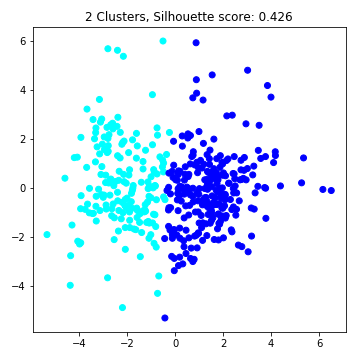
\includegraphics{img/kmeans_fav.png}
\caption{K-Means}
\end{figure}

    The `K-Means' image is the result of K-Means clustering. In this case,
the first principal component (which cares Detergent\_Paper) slices the
customers into two (into two groups of course). So, labeling the data
set according to the Detergent\_Paper spendings like
Detergent\_Paper\_Customer = 1 if the customer is in the left group and
0 otherwise may lead us a new supervised data set. Then further work
should be maintained in the supervised area as new customers appears on
the data set by time.

    \begin{figure}[!h]
\centering
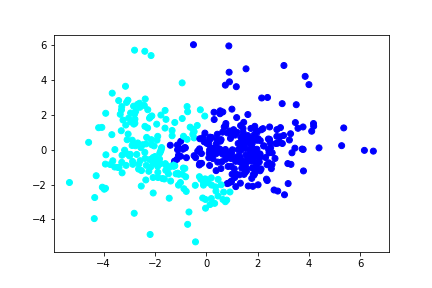
\includegraphics{img/hierarchical_fav.png}
\caption{Hierarchical}
\end{figure}

    The `Hierarchical' is the result of hierarchical clustering. Similar to
result of K-Means algorithm but, this one tends to assign customers who
are likely to spend on Fresh and Frozen categories and less likely to
spend on Detergents\_Paper category to the left group.

Something similar happens to those customers who tend to spend on
Detergents\_Paper but not likely to spend on Fresh and Frozen too much.

According to this figure, same labeling with K-Means can be made on the
data set for the further work.

Altough this clustering was the best choice according to its dendrogram,
this one is also interesting (Hierarchical 2):

    \begin{figure}[!h]
\centering
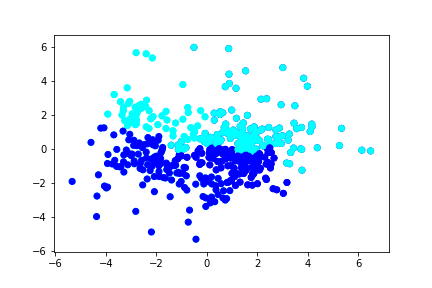
\includegraphics{img/hierarchical_fav2.png}
\caption{Hierarchical 2}
\end{figure}

    Roughly, it separates the customers by the second principal component.
Maybe not very convenient but, as an alternative, the data set may be
labeled with customers' Fresh and Frozen spendings. Then the problem
becomes a supervised one again.

    \begin{figure}
\centering
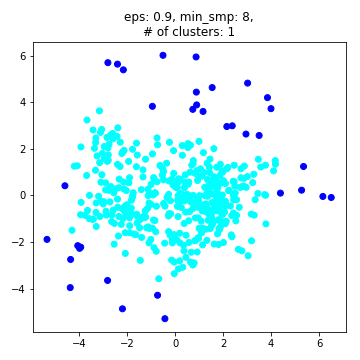
\includegraphics{img/dbscan_fav.png}
\caption{Dbscan}
\end{figure}

    `Dbscan` grouped the dense fields on the plane. According to the result,
there is a big group of customers whose spending habits are similar.
Whereas there are outliers around it, who have spending habits different
than this big group. The wholesale distributor may count them as special
customers and treat them differently according to their special spending
habits.


    % Add a bibliography block to the postdoc
    
    
    
    \end{document}
